\section{Fast iterative solver using Wirtinger's framework}
\label{sec:Solver}

\begin{figure*}[t!]
\begin{center}
\includegraphics[width=\textwidth]{\FigDir ConvergenceLog.pdf}
%\includegraphics[width=\textwidth]{\FigDir ConvergenceLog.eps}
\caption{\label{fig:Convergence} This plot shows the amplitude (top
  panels) and
  phase (bottom panels) of the difference between
  the estimated gains and the true (random) gains in the different
  directions for the different antenna (shaded greys full lines).}
\end{center}
\end{figure*}

This section describes a Levenberg-Maquardt based calibration algorithm, using
Wirtinger derivative to define the Jacobian (the \COH~algorithm, see
Sec. \ref{sec:COH}). This problem is addressed in greater detail in \citet[][]{SmirnovTasse14}.

\subsection{Levenberg-Maquardt}

In the following $h$ is the non-linear operator mapping the
4-polarisations, direction-dependent gain vector $\vec{g}$ to the
visibility vector $\vis$ containing all baselines, time and frequency
data

\begin{alignat}{2}
\vis=h\left(\vec{g}\right)=&
\begin{bmatrix} 
\vdots \\ 
h_{pq}\left(\vec{g}\right)\\ 
\vdots \\ 
\end{bmatrix}
\end{alignat}


\noindent where $h_{pq}$ is defined in Eq. \ref{eq:hpq}.

The direction-dependent Jones matrices appearing in the measurement
equation (Eq. \ref{eq:ME}) can then be estimated using a chi-square
minimisation technique such as the Levenberg-Maquardt. Specifically, the gain vector $\vec{g}$ can be iteratively estimated from the
measured visibilities $\mathbf{v_m}$ as

\def\SimpleJacobAtXi{\bm{J}\big|_{\widehat{\g_{i}}}}
\def\HAtXi{\H\big|_{\widehat{\g_{i}}}}
\def\KAtXi{\textbf{K}\big|_{\widehat{\g_{i}}}}
\begin{alignat}{2}
\label{eq:LM}
\widehat{\vec{g}_{i+1}}=&\widehat{\vec{g}_{i}}+\KAtXi^{-1}\SimpleJacobAtXi^H\textbf{C}^{-1}\left(\mathbf{v_m}-h\left(\widehat{\vec{g}_{i}}\right)\right)\\
\text{with }\KAtXi=&\HAtXi+\lambda.\text{diag} \left(\HAtXi\right)\\
\text{and }\HAtXi=&\SimpleJacobAtXi^H\textbf{C}^{-1}\SimpleJacobAtXi
\end{alignat}

\noindent where the matrix $\SimpleJacobAtXi$ is the Jacobian of $h$
estimated at $\widehat{\g_{i}}$, and
$\textbf{C}$ is the covariance matrix of $\mathbf{v}$.

The Levenberg-Maquardt algorithm can be equivalently applied by using the Wirtinger Jacobian
or the classical Jacobian. In this paper, as mentioned in Sec. \ref{sec:Wirtinger}, instead of computing the Jacobian using the real and
imaginary parts of gains as independent variables, we use the Wirtinger
derivative definition (see Sec. \ref{sec:WirtingerJacob})

\begin{alignat}{2}
\label{eq:LMWirtinger}
\SimpleJacob:=&\JV
\end{alignat}

\subsection{The \COH~algorithm}
\label{sec:COH}

The Wirtinger $\SimpleJacob^H\SimpleJacob$ has a different structure to the classical one. In this section, we describe an algorithms that uses {\it only one} of the
two independent Wirtinger variable (either $z$ or $\conj{z}$). In
short, in this section $\SimpleJacob$ is reduced to

\begin{alignat}{2}
\label{eq:LMWirtinger}
\SimpleJacob:=&\JVg
\end{alignat}

\noindent which means only half of the
Jacobian $\JV$ is used, and a single principal block in the matrix
$\JV^H\JV$ is constructed (see Fig. \ref{fig:HalfJHJ}). The algorithm is referred to {\it Complex Half-Jacobian Optimization for
N-directional EStimation} (\COH).

Intuitively, the idea relies on that the RIME (Eq. \ref{eq:ME}) has the remarkable property to
behaves like a linear system around the solution. Specifically, from Eq. \ref{eq:Jpq0} and
\ref{eq:Jpq1}, it is easy to check that:

\begin{alignat}{2}
\label{eq:Lin}
\vis=&\frac{1}{2}\left(\JV\big|_{\gwirt}\right)\ \gwirt
\end{alignat}

\noindent while

\begin{alignat}{2}
\label{eq:Lin2}
\vis=&h\left(\vec{g}\right)=\left(\JVg\big|_{\conj{\g}}\right)\ \g\\
\text{and }\vis=&\left(\JVCg\big|_{\g}\right)\ \conj{\g}
\end{alignat}

%% \begin{alignat}{2}
%% \label{eq:Lin}
%% \mathbf{v}=\left(\JV\big|_{\vec{g}}\right).\vec{g}
%% \end{alignat}

%% \noindent where $\JV\big|_{\vec{g}}$ mean that the Jacobian is
%% evaluated at $\vec{g}$.

Both Eq. \ref{eq:Lin} and \ref{eq:Lin2} form linear
systems. Furthermore it is shown in \citet[][]{SmirnovTasse14}
that the principal blocks of $\JV^H\JV$ corresponding to the
$(\vec{g},\conj{\vec{g}})$ and $(\conj{\vec{g}},\vec{g})$ cross
terms have a smaller amplitude than the $(\vec{g},\vec{g})$ and
$(\conj{\vec{g}},\conj{\vec{g}})$ blocks.


\begin{figure}[h!]
\begin{center}
\includegraphics[width=\columnwidth]{\FigDir NewHalfJHJ.pdf}
\caption{\label{fig:HalfJHJ} This figure shows amplitude (left panel)
  and phase (right panel) of the block-diagonal matrix $\JVg^H\JVg$
  for the dataset described in the text. Each block corresponds to the
different directions for each specific antenna. Its block structure
make it easily invertible.}
\end{center}
\end{figure}

\begin{figure*}[t!]
\begin{center}
%\hspace*{-1.3cm}
%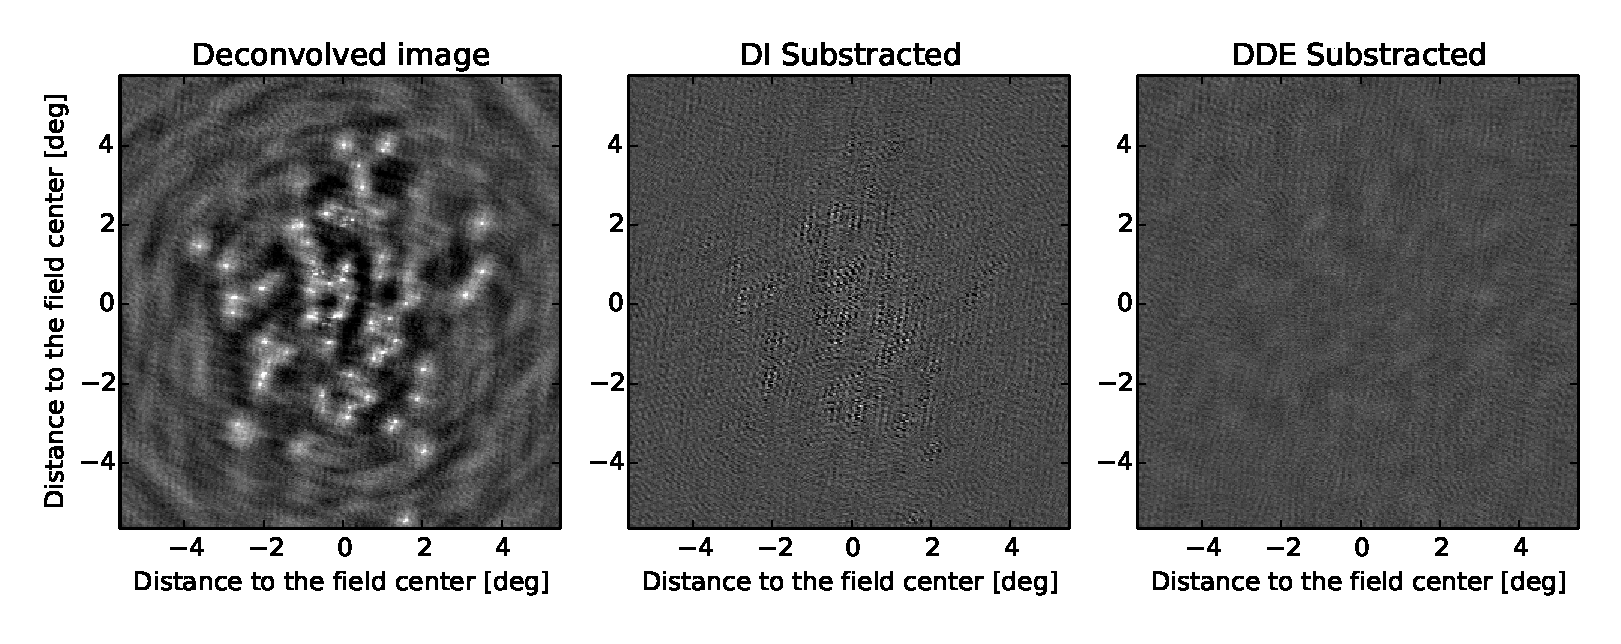
\includegraphics[width=\textwidth]{residSim.eps}
%\includegraphics[width=\textwidth]{\FigDir residSimZoom2.eps}
\includegraphics[width=\textwidth]{\FigDir Pealed.pdf}
\caption{\label{fig:resid} This figure shows the comparison between
  the deconvoled image
  (left), the residuals data after simple skymodel subtractions
  (center), and the residuals data after subtracting the
  sky model corrupted by the direction-dependent \COH~estimated solution
  (right). The color scale is the same in all panels. In this
  simulation, \COH~reduces the
residual data level by a factor of $\sim30$.}
\end{center}
\end{figure*}


The structure of $\JVg^H\JVg$ is shown in Fig. \ref{fig:HalfJHJ} for
the dataset described in Sec. \ref{sec:SimpleSimul}. This
matrix is block diagonal, essentially because 
$\partial \conj{g}/\partial g=0$ in Wirtinger's framework. This allows
for dramatic improvement in algorithmic cost, as the $\JV^H\JV$ matrix
inversion cost is $\mathcal{O}\left(n_d^3n_a\right)$ instead of being
$\mathcal{O}\left(n_d^3n_a^3\right)$ corresponding to a net gain of $n^2_a$.
% In the same manner, the
% matrix product $\textbf{K}^{-1}\SimpleJacob^H$ as well as the
% computation of $\JV^H\JV$ are $n^2_a$ times cheaper.

Another interesting property is that, assuming
$\text{diag}\left(\H\right)\approx\H$ and injecting Eq. \ref{eq:Lin2}
into Eq. \ref{eq:LM}, we find:

\def\Fact{\left(\lambda+1\right)^{-1}}
\def\ThisJ{\JVg\big|_{\conj{\widehat{\g_{i}}}}}
\begin{alignat}{2}
\label{eq:HalfLM}
\widehat{\vec{g}_{i+1}}=&\lambda\Fact\widehat{\vec{g}_{i}}+\Fact\H_{\widehat{\vec{g}_{i}}}^{-1}\ThisJ^H\textbf{C}^{-1}\mathbf{v_m}\\
\text{with }\H_{\vec{g}}=&\ThisJ^H\textbf{C}^{-1}\ThisJ
\end{alignat}

\noindent meaning the predict step does not have to be computed along
the iteration.

%% \subsection{Convergence and averaging}

%% As shown in Fig. ... the convergence of this algorithm is slow, and
%% following Stef-the-great, instead of estimating $\JV$ at
%% $\widehat{\vec{g}_i}$, we build it at a modified location constructed
%% from previous iterations, and Eq. \ref{eq:SolveA} becomes:

%% \begin{alignat}{2}
%% \A=&\JV\big|_{\widetilde{\vec{g}_i}}\\
%% \text{with } \widetilde{\vec{g}_i}=&(\widehat{\vec{g}_{i-1}}+\widehat{\vec{g}_{i}})/2
%% \end{alignat}


